% Options for packages loaded elsewhere
\PassOptionsToPackage{unicode}{hyperref}
\PassOptionsToPackage{hyphens}{url}
%
\documentclass[
  12pt,
]{article}
\usepackage{amsmath,amssymb}
\usepackage{iftex}
\ifPDFTeX
  \usepackage[T1]{fontenc}
  \usepackage[utf8]{inputenc}
  \usepackage{textcomp} % provide euro and other symbols
\else % if luatex or xetex
  \usepackage{unicode-math} % this also loads fontspec
  \defaultfontfeatures{Scale=MatchLowercase}
  \defaultfontfeatures[\rmfamily]{Ligatures=TeX,Scale=1}
\fi
\usepackage{lmodern}
\ifPDFTeX\else
  % xetex/luatex font selection
\fi
% Use upquote if available, for straight quotes in verbatim environments
\IfFileExists{upquote.sty}{\usepackage{upquote}}{}
\IfFileExists{microtype.sty}{% use microtype if available
  \usepackage[]{microtype}
  \UseMicrotypeSet[protrusion]{basicmath} % disable protrusion for tt fonts
}{}
\makeatletter
\@ifundefined{KOMAClassName}{% if non-KOMA class
  \IfFileExists{parskip.sty}{%
    \usepackage{parskip}
  }{% else
    \setlength{\parindent}{0pt}
    \setlength{\parskip}{6pt plus 2pt minus 1pt}}
}{% if KOMA class
  \KOMAoptions{parskip=half}}
\makeatother
\usepackage{xcolor}
\usepackage[margin=2cm]{geometry}
\usepackage{graphicx}
\makeatletter
\def\maxwidth{\ifdim\Gin@nat@width>\linewidth\linewidth\else\Gin@nat@width\fi}
\def\maxheight{\ifdim\Gin@nat@height>\textheight\textheight\else\Gin@nat@height\fi}
\makeatother
% Scale images if necessary, so that they will not overflow the page
% margins by default, and it is still possible to overwrite the defaults
% using explicit options in \includegraphics[width, height, ...]{}
\setkeys{Gin}{width=\maxwidth,height=\maxheight,keepaspectratio}
% Set default figure placement to htbp
\makeatletter
\def\fps@figure{htbp}
\makeatother
\setlength{\emergencystretch}{3em} % prevent overfull lines
\providecommand{\tightlist}{%
  \setlength{\itemsep}{0pt}\setlength{\parskip}{0pt}}
\setcounter{secnumdepth}{-\maxdimen} % remove section numbering
\ifLuaTeX
\usepackage[bidi=basic]{babel}
\else
\usepackage[bidi=default]{babel}
\fi
\babelprovide[main,import]{brazilian}
% get rid of language-specific shorthands (see #6817):
\let\LanguageShortHands\languageshorthands
\def\languageshorthands#1{}
\usepackage[utf8]{inputenc}
\usepackage{caption}
\captionsetup{labelfont=bf}
\usepackage{float}
\ifLuaTeX
  \usepackage{selnolig}  % disable illegal ligatures
\fi
\usepackage{bookmark}
\IfFileExists{xurl.sty}{\usepackage{xurl}}{} % add URL line breaks if available
\urlstyle{same}
\hypersetup{
  pdfauthor={Isabelle Fernandes de Oliveira Sannier},
  pdflang={pt-BR},
  hidelinks,
  pdfcreator={LaTeX via pandoc}}

\author{Isabelle Fernandes de Oliveira Sannier}
\date{}

\begin{document}

\begin{titlepage}
\centering

{\large Universidade Federal de Minas Gerais (UFMG) \par}
\vspace{0.5cm}

{\large Departamento de Ciência da Computação \par}
\vspace{4cm}

{\large Isabelle Fernandes de Oliveira Sannier (2021432208)\par}
\vspace{5cm}

{\Large \textbf{Trabalho Prático 3: Consultas ao Sistema Logístico} \par}
\vspace{10cm}

{\large Belo Horizonte, 06 de julho de 2025 \par}


\end{titlepage}

\subsection{1. Introdução}\label{introduuxe7uxe3o}

Este trabalho tem como objetivo desenvolver um sistema de consultas para
processar e extrair informações de um grande volume de dados gerados
pela operação logística dos Armazéns Hanoi. O desafio principal consiste
em processar um arquivo de entrada cronológico que intercala
atualizações de estado de pacotes e consultas, respondendo a estas em
tempo real com base nas informações disponíveis até aquele momento.

Dois tipos principais de consulta são o foco: o levantamento do
histórico completo de um pacote específico (consulta PC) e a recuperação
do estado atual de todos os pacotes associados a um determinado cliente
(consulta CL). O desafio computacional reside em responder a estas
consultas de forma eficiente, sem a necessidade de varrer todo o banco
de dados a cada nova requisição, o que seria inviável para um grande
volume de eventos.

Para isso, a solução adotada baseia-se na construção de um sistema de
indexação em memória. Foram projetadas e implementadas múltiplas Árvores
AVL, uma estrutura de dados de busca auto-balanceada, para criar os
índices necessários. Um índice primário (IndicePacotes) mapeia o
identificador de cada pacote ao seu histórico completo de eventos,
permitindo acesso rápido para a consulta PC. Um segundo índice, mais
complexo (IndiceClientes), mapeia o nome de cada cliente a uma estrutura
de dados secundária que mantém seus pacotes sempre ordenados pelo tempo
do evento mais recente. Esta arquitetura permite que as consultas sejam
resolvidas com complexidade de tempo logarítmica, garantindo o alto
desempenho exigido pelo problema.

\subsection{2. Método}\label{muxe9todo}

A solução foi estruturada de forma modular, com um laço de processamento
principal na função main que orquestra a interação entre um banco de
dados em memória e um conjunto de índices de alto desempenho. A cada
linha lida do arquivo de entrada, o sistema ou atualiza sua base de
dados com um novo evento ou utiliza os índices para responder a uma
consulta.

\textbf{Classe BancoDados:} Atua como o repositório central para todos
os eventos da simulação. Internamente, utiliza um array dinâmico que
armazena ponteiros para os objetos Evento (Evento**). Esta abordagem de
indireção é crucial para a robustez do sistema: os objetos Evento são
alocados individualmente na memória Heap e seus endereços permanecem
estáveis e imutáveis durante toda a execução. Assim, mesmo que o array
de ponteiros precise ser redimensionado, os ponteiros guardados na
estrutura ListaPacotesClientes nunca se tornam inválidos, garantindo a
integridade de todo o sistema de indexação. A classe também possui um
mecanismo de redimensionamento para lidar com um volume arbitrário de
eventos.

\textbf{Classe Evento:} Representa um único registro do log de
operações. A classe foi projetada para conter todos os campos possíveis
de qualquer tipo de evento (RG, AR, TR, etc.). Para garantir a segurança
da memória, especialmente para os nomes de clientes alocados
dinamicamente (char*), a classe implementa a ``Regra dos Três''
(Destrutor, Construtor de Cópia e Operador de Atribuição de Cópia),
assegurando que cópias de objetos Evento sejam sempre profundas e
seguras.

\textbf{Classe ArvoreAVLPacote:} O primeiro índice, projetado para
responder eficientemente à consulta PC. Foi implementado como uma Árvore
AVL, uma árvore de busca binária auto-balanceada.

\begin{itemize}
\item
  Chave: O id do pacote (um int).
\item
  Valor: Uma Fila contendo os índices de todos os eventos associados
  àquele pacote no BancoDados principal. A cada novo evento de um
  pacote, seu índice é simplesmente adicionado ao final da fila do nó
  correspondente. O indice corresponde a um int que remete a posicao
  daque evento ao vetor de eventos no banco de dados.
\end{itemize}

\textbf{Classe ArvoreAVLClientes:} Seria uma ``Árvore de Listas
encadeada'', mais complexo que o índice pacotes, projetado para a
consulta CL. Para atender ao requisito de ordenação por tempo, foi
implementado com uma arquitetura de dois níveis:

\begin{itemize}
\item
  ArvoreAVLClientes: A árvore principal, também uma AVL, mapeia o nome
  de um cliente (std::string) a um ponteiro para uma estrutura de dados
  secundária.
\item
  ListaPacotesCliente: A estrutura secundária, implementada como uma
  lista encadeada ordenada. Cada nó nesta lista representa um pacote
  associado ao cliente e armazena um ponteiro para o primeiro evento e o
  último evento conhecido daquele pacote. A lista é mantida
  perpetuamente ordenada pelo tempo deste último evento, através de um
  método atualiza que remove a entrada antiga do pacote e re-insere a
  nova em sua posição ordenada correta.
\end{itemize}

\textbf{Algoritmos e Fluxo Principal:} O laço principal na main lê cada
linha e seu identificador (EV, PC ou CL).

Ao processar um EV: Uma função ``fábrica'' (criar\ldots) correspondente
é chamada para criar o objeto Evento. Este é adicionado ao BancoDados, e
os dois índices são atualizados. A atualização do IndiceClientes utiliza
uma lógica de busca cruzada: ela primeiro consulta o IndicePacotes para
descobrir quem são o remetente e o destinatário originais daquele
pacote, para então atualizar as listas ordenadas de ambos os clientes
com o novo evento.

Ao processar uma consulta (PC ou CL): O sistema realiza uma busca rápida
no índice apropriado. Para a consulta CL, a ListaPacotesCliente
resultante é percorrida em ordem, já que ela se mantém sempre ordenada,
gerando a resposta de forma eficiente, sem a necessidade de ordenação no
momento da consulta.

\subsection{3. Análise de
Complexidade}\label{anuxe1lise-de-complexidade}

O desempenho do sistema de consultas é determinado pela eficiência das
estruturas de dados de indexação durante o processamento do arquivo de
entrada, que contém um total de M linhas. A análise foca nas duas
operações principais: a atualização dos índices a cada evento (EV) e a
execução das consultas (PC e CL).

\textbf{Operações de Atualização (por Evento EV):}

A cada evento lido, são realizadas operações de busca e inserção nos
índices pacote e cliente. Quando um evento novo chega ele é indexado na
ArvoreAVLPacotes com complexidade \(O (log\ P)\), onde P é o número de
pacotes únicos.

Busca na Árvore de Clientes: A busca por um cliente na ArvoreAVLClientes
envolve um passo anterior, que é saber os clientes envolvidos (remetente
e destinatario). Para isso, a descoberta dos clientes envolve
complexidade \(O (log\ P)\) novamente, da forma que foi implementado,
pois uma busca pelo id do pacote é feita e capturado essas duas
variáveis (remetente e destinatário). Com essa informação, é feito uma
busca na ArvoreAVLCliente com complexidade de tempo
\(2\cdot O (log\ C)\), onde C é o número total de clientes únicos.

Atualização da Lista de Pacotes: A operação de atualiza na
ListaPacotesCliente (que envolve remover e reinserir de forma ordenada)
tem complexidade de tempo, no pior caso (quando o evento final a ser
atualizado é removido e inserido estão no fim da lista encadeada) é
\(2 \cdot O(P_c)\) (um para remover e outro para inserir), onde \(P_c\)
é o número de pacotes associados àquele cliente específico.

Portanto, o custo para processar um único evento EV é assintoticamente
\(O(log\ P + log\ C+ P_c)\).

\textbf{Operações de Consulta:}

Consulta por Pacote (PC): Envolve uma busca na ArvoreAVLPacote, com
custo \(O (log\ P)\), onde P é o número de pacotes únicos. Em seguida,
percorre a fila de resultados, com custo \(O(E_p)\), onde \(E_p\) é o
número de eventos para aquele pacote. Complexidade total:
\(O(log\ P + E_p)\).

Consulta por Cliente (CL): Envolve uma busca na ArvoreAVLClientes
\(O(log\ C)\). A etapa seguinte, em imprimeResultados, percorre os
\(P_c\) eventos armazenados na lista encadeada já ordenada e imprime, o
que tem um custo de \(O(P_c)\). Complexidade total: \(O(log\ C + P_c)\).

\textbf{Complexidade Geral:}

Complexidade de Tempo: É o somatório dos custos de todas as M operações
no arquivo de entrada. Para formalizar, define-se \(Me_{ev}\),
\(M_{pc}\) e \(M_{cl}\) como o número de operações de evento, consulta
de pacote e consulta de cliente, respectivamente, onde
\(M = M_{ev} + M_{pc} + M_{cl}\).

O custo total pode ser expresso como:
\(T(M)=M_{ev} \cdot O(logP+logC+Pc) + M_{pc} \cdot O(logP+Ep) + M_{cl} \cdot O(logC+Pc)\)

A complexidade de espaço é determinada pelo armazenamento dos eventos e
dos índices: \(O(E+P+C)\), onde E é o número total de eventos
armazenados, P é o número de nós no índice de pacotes e C é o número de
nós no índice de clientes.

\subsection{4. Estratégias de
Robustez}\label{estratuxe9gias-de-robustez}

\textbf{Gerenciamento de Memória e a Regra dos Três:} A classe Evento,
que gerencia memória alocada dinamicamente para os nomes de remetente e
destinatário (char*), implementa a ``Regra dos Três''. Foram criados um
Construtor de Cópia e um Operador de Atribuição de Cópia customizados
para realizar cópias profundas (deep copies). Isso garante que cada
objeto Evento tenha sua própria memória, eliminando completamente os
erros de double free e use-after-free que surgem de cópias rasas.

\textbf{Limpeza Encadeada de Memória:} Os destrutores de todas as
classes que alocam memória foram implementados para liberar os recursos.
Notavelmente, o destrutor da ArvoreAVLClientes é responsável por deletar
os ponteiros para as ListaPacotesCliente que armazena, e o destrutor de
cada lista, por sua vez, deleta os nós que a compõem, criando uma cadeia
segura de descarte de memória.

\textbf{Validação de Entrada:} O programa valida as entradas externas.
Na main, o código verifica se o número correto de argumentos de linha de
comando foi fornecido (if (argc \textless{} 2)). Imediatamente após, ele
também verifica se o arquivo de entrada pôde ser aberto com sucesso (if
(!arquivo\_entrada.is\_open())), tratando os dois casos de erro mais
comuns antes de iniciar o processamento. Além disso, verifica-se se o
tempo da consulta de cliente ou pacotes correspondem ao ocorrido. Foi
verificado, na fase de análise experimental que algumas consultas
clientes/pacotes eram inválidas, ou seja, perguntava-se sobre um id de
pacote que ocorreria somente no futuro. Da mesma forma, perguntava-se
por um cliente que ainda não havia ocorrido.

\textbf{Arrays Dinâmicos:} Para garantir que a estrutura
ListaPacotesCLientes, que apontam para os eventos, não se tornasse
inválida quando o BancoDados redimensionasse seu array interno, foi
adotada uma arquitetura de indireção. O banco de dados não armazena os
objetos Evento diretamente, mas sim um array de ponteiros para Evento.
Dessa forma, os objetos Evento têm um endereço de memória fixo durante
toda a vida do programa. A operação de redimensionamento do banco de
dados copia apenas os ponteiros --- uma operação rápida --- e não
invalida as referências mantidas pelos índices, tornando o sistema imune
a erros de ``ponteiros fantasmas'' (dangling pointers) causados por
realocação de memória.

\textbf{Uso da Ferramenta Valgrind:} Durante todo o ciclo de
desenvolvimento, a ferramenta de análise de memória Valgrind foi
utilizada para inspecionar o uso da memória. O programa foi ajustado
iterativamente até que o Valgrind reportasse uma execução limpa, sem
vazamentos de memória (leaks), erros de leitura/escrita ou outros
problemas de gerenciamento de memória.

\subsection{5. Análise Experimental}\label{anuxe1lise-experimental}

Para a avaliação de desempenho do sistema logístico, foi realizada uma
análise experimental. A metodologia consistiu em gerar cenários de
simulação variando sistematicamente um parâmetro de entrada por vez,
enquanto os demais eram mantidos em valores fixos. Este controle permite
isolar e observar o impacto de cada variável individualmente no
comportamento do sistema. O script em R foi utilizado para gerar os
cenários, empregando sorteios aleatórios sem reposição para garantir a
diversidade dos valores em cada experimento.

As medidas escolhidas para variar foram:

\begin{itemize}
\item
  Quantidade de Pacotes: Foram realizados 300 sorteios sem reposição,
  com valores variando de 10 a 900 pacotes.
\item
  Quantidade de Clientes: Foram realizados 300 sorteios sem reposição,
  com valores variando de 10 a 2.000 clientes.
\item
  Capacidade de Transporte: Foram realizados 300 sorteios sem reposição,
  com valores de capacidade variando de 1 a 300.
\end{itemize}

Conforme a metodologia, enquanto uma variável era alterada, as outras
permaneciam fixas. Os valores padrão utilizados foram:

\begin{itemize}
\item
  Quantidade de Pacotes: 500.
\item
  Quantidade de Clientes: 500.
\item
  Capacidade de Transporte: 50.
\item
  Número de Armazéns (nós): 10.
\end{itemize}

Ao todo, foram gerados 900 cenários diferentes, divididos em 300
experimentos para cada uma das três variáveis analisadas. As métricas de
desempenho adotadas para esta análise focaram no tempo de execução
computacional das principais operações de busca do sistema:

\begin{itemize}
\item
  Tempo de Consulta por Pacote (PC): O tempo, em nanossegundos,
  necessário para buscar e retornar todos os eventos associados a um
  identificador de pacote específico.
\item
  Tempo de Consulta por Cliente (CL): O tempo, em nanossegundos,
  necessário para buscar e retornar o histórico completo de pacotes
  associados a um nome de cliente específico.
\end{itemize}

Abaixo, seguem os gráficos gerados a partir dos dados de tempo coletados
para cada tipo de consulta.

\begin{figure}[H]

{\centering 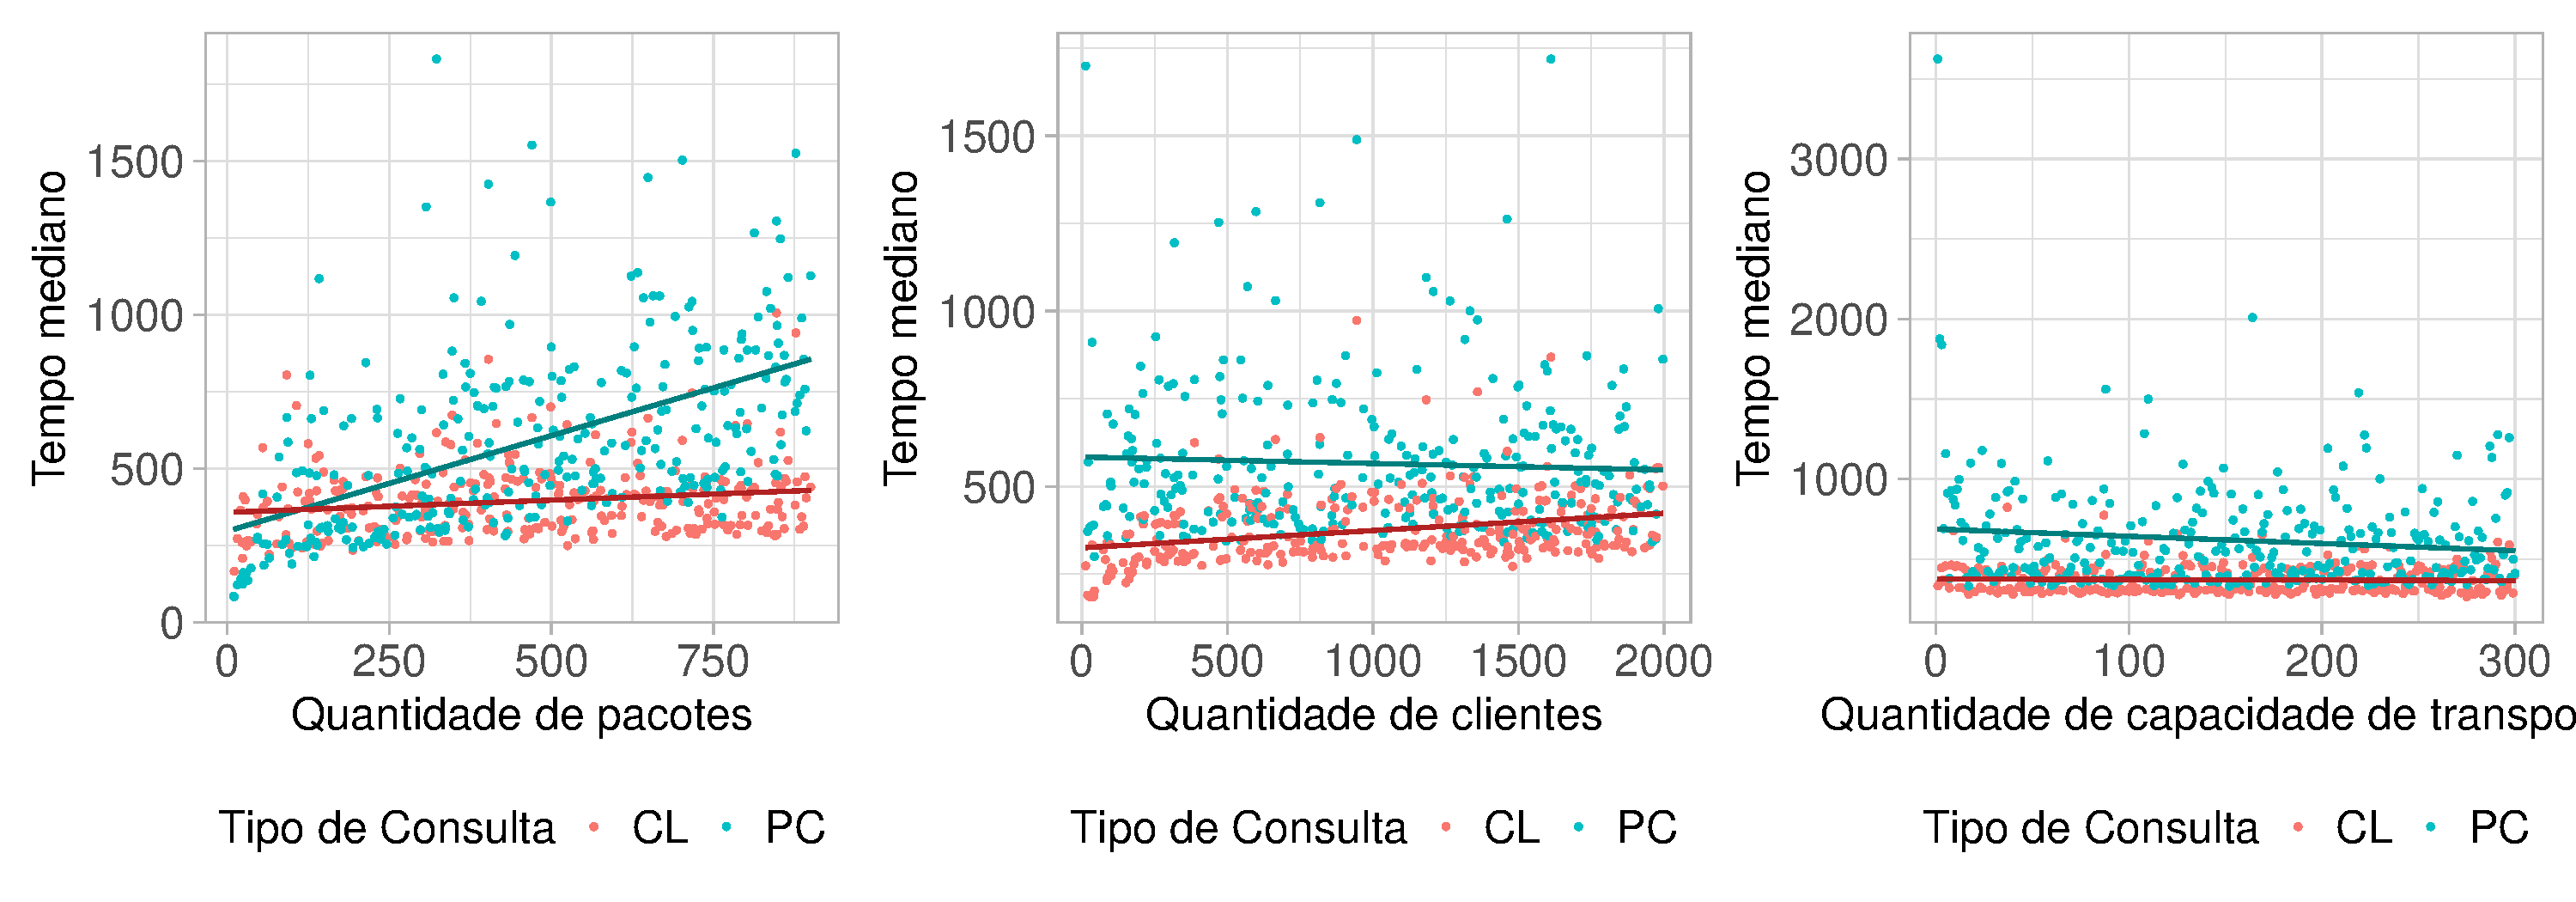
\includegraphics{Relatorio_files/figure-latex/grafico rearmazenado-1} 

}

\caption{\textbf{Análise de desempenho das consultas CL e PC em diferentes cenários de entrada}}\label{fig:grafico rearmazenado}
\end{figure}

A Figura 1 apresenta três gráficos de dispersão que comparam o tempo de
execução de dois tipos de consulta, consulta cliente (CL) e consulta
pacote (PC), em relação a diferentes variáveis: quantidade de pacotes,
quantidade de clientes e quantidade de capacidade de transporte. Cada
gráfico inclui uma linha de tendência que ajuda a visualizar o
comportamento mediano do tempo em função das variáveis analisadas.

No primeiro gráfico, observa-se que à medida que a quantidade de pacotes
aumenta, o tempo de execução da consulta PC também cresce de forma
acentuada. A linha de tendência revela uma inclinação positiva
significativa, indicando que essa consulta é bastante sensível ao
aumento dessa variável. Por outro lado, a consulta CL apresenta um
crescimento mais suave do tempo em relação à quantidade de pacotes, com
uma linha de tendência levemente inclinada. Isso ocorre porque o número
de clientes está fixado em 500, então o índice cliente é constante.

No segundo gráfico, que relaciona a quantidade de clientes com o tempo
mediano de execução, percebe-se que o tempo da consulta CL tende a
aumentar levemente com o número de clientes. Já a consulta PC apresenta
uma linha praticamente horizontal, ou até mesmo com leve inclinação
negativa, o que indica que o tempo mediano permanece estável --- ou até
melhora --- com o aumento no número de clientes. Essa estabilidade é
justificada pelo fato do número de pacotes estar fixado em 500, então o
índice pacotes é constante.

O terceiro gráfico analisa a quantidade de capacidade de transporte em
relação ao tempo mediano. Nesse caso, tanto a consulta CL quanto a PC
apresentam linhas de tendência praticamente horizontais, o que indica
que essa variável tem pouca ou nenhuma influência sobre o tempo de
execução de ambas as consultas. Portanto, pode-se concluir que a
quantidade de capacidade de transporte não é um fator relevante na
performance dos algoritmos analisados. Essa variável foi escolhida
pensando que, se a capacidade de transporte fosse menor, mais eventos de
rearmazenamento ocorreria, ocasionando em um maior número de eventos,
que por sua vez, impactaria no tempo de execução do algoritmo. Contudo,
esse impacto é até ocorre, mas são nos momentos de atualização dos
indices (pacote ele acrescenta mais um evento para o respectivo id e
clientes ele atualiza o último evento do pacote). Contudo essas
atualizações acontecem no tempo de processamento de leitura das
variáveis. Como o intuito é mensurar o tempo de consulta e não o tempo
de leitura, o impacto da quantidade de eventos não interfere no tempo de
consulta. Isso é um pouco lógico, pois a consulta está diretamente
relacionada com a altura das árvores AVL (estruturas escolhidas para os
índices pacotes e clientes). Logo, o número de pacotes e o número de
clientes que interfere na altura da árvore.

\newpage

\subsection{6. Conclusão}\label{conclusuxe3o}

O presente trabalho se propôs a desenvolver e analisar um sistema de
consultas de alto desempenho, projetado para processar um grande volume
de eventos logísticos dos Armazéns Hanoi em tempo real. O objetivo
central foi criar uma solução capaz de responder eficientemente a
consultas sobre o histórico de pacotes (PC) e o estado atual dos pacotes
de clientes (CL), a fim de evitar varreduras completas do banco de dados
a cada requisição.

A implementação do projeto em C++ proporcionou um aprendizado prático na
aplicação de estruturas de dados para a resolução de um problema
complexo de indexação. O uso de Árvores AVL auto-balanceadas foi a
solução adotada, garantindo buscas, inserções e remoções com
complexidade logarítmica. Para a consulta CL, uma arquitetura de dois
níveis, combinando uma ArvoreAVLClientes com a estrutura
ListaPacotesCliente (uma lista encadeada ordenada), mostrou-se uma
solução elegante e eficiente para manter os pacotes de cada cliente
sempre ordenados pelo evento mais recente, eliminando a necessidade de
ordenação no momento da consulta. Adicionalmente, a adoção de uma
arquitetura de indireção no BancoDados, armazenando ponteiros para os
eventos, foi crucial para garantir a robustez e a segurança da memória
contra ponteiros inválidos.

A arquitetura do sistema foi centralizada na função main, que atua como
um controlador principal. Este laço de processamento orquestra a leitura
do arquivo de entrada e delega as tarefas de forma eficiente: ou
atualizando os índices ao receber um novo evento (EV) ou utilizando-os
para executar uma busca e responder a uma consulta (PC ou CL).

Por fim, a Análise Experimental validou o desempenho e a escalabilidade
da solução de indexação. Ao variar sistematicamente os parâmetros que
governam o tamanho dos índices --- a quantidade de pacotes e de clientes
---, foi possível confirmar experimentalmente a análise de complexidade
teórica. Os resultados demonstraram que o tempo de consulta está
diretamente correlacionado ao tamanho da respectiva árvore de índice,
enquanto outras variáveis operacionais, como a capacidade de transporte,
tiveram impacto desprezível no tempo de busca.

\newpage

\subsection{7. Referência}\label{referuxeancia}

LACERDA, Anisio; MEIRA JR., Wagner; CUNHA, Washington. Estruturas de
Dados. Slides da disciplina DCC205 -- Estruturas de Dados, Departamento
de Ciência da Computação, ICEx/UFMG, 2025.

UNIVERSIDADE FEDERAL DE MINAS GERAIS. Departamento de Ciência da
Computação. Especificação do Trabalho Prático -- Consultas ao Sistema
Logístico. Belo Horizonte: DCC/ICEx/UFMG, 2025. Documento em PDF.

\end{document}
